\chapter{The First 16\textsuperscript{4} Theme Tunes} 

It's possible to dig into the making of the title music and how Jeff Minter
arrived the music configuration he did thanks to a number of tiny demo programs that
survive from the period when he was developing Iridis Alpha.

Jeff distributed these on Compunet in the summer of 1986.

It turns out he was inspired by an article in 'Byte' magazine from June 1986 that
described how to make 'Fractal Music'. This article outline a version of the
algorithm that Jeff ultimately adopted. The 'self-similarity' we encountered
in the way the Iridis Alpha theme tunes are constructed, a four-note structure
repeated across different time intervals on each of the three voices, finds its
roots in this article.


\begin{figure}[H]
{
  \begin{adjustbox}{width=11cm,center}
  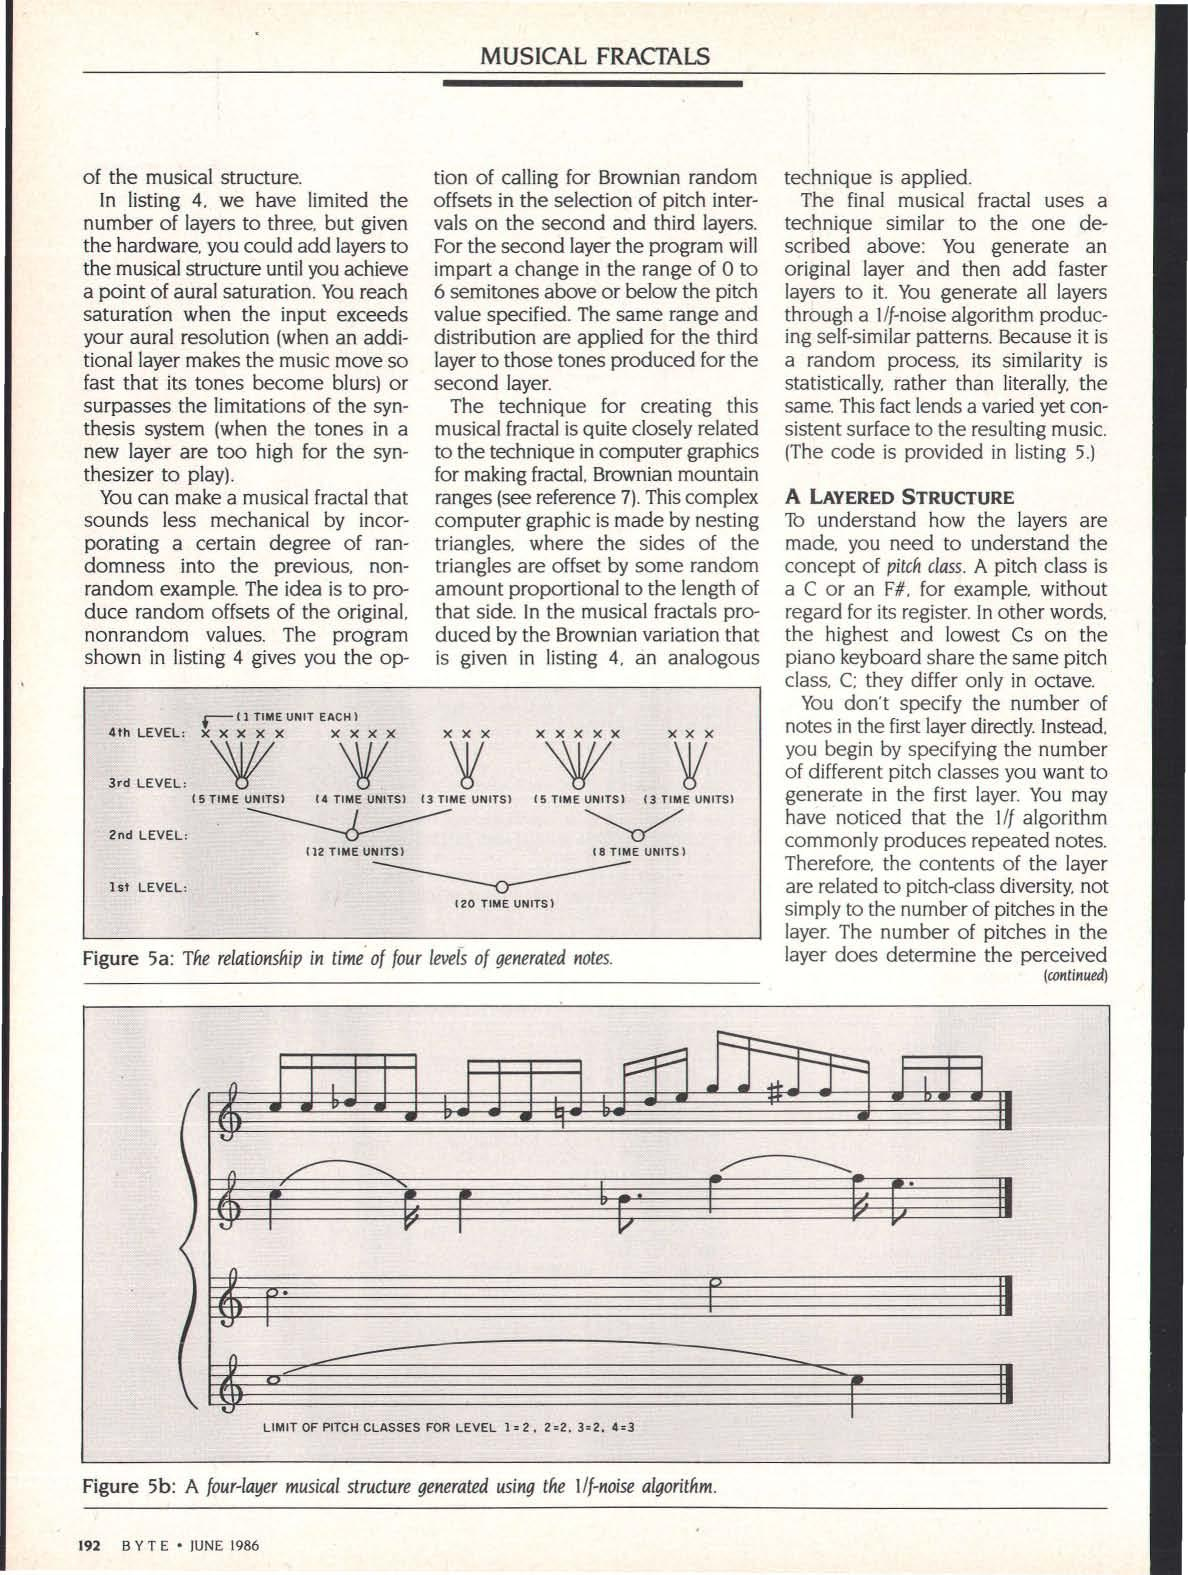
\includegraphics[width=11cm]{torus/fractal.jpg}%
    \end{adjustbox}
}\caption[]{}
\end{figure}


\subsection{Taurus:Torus}
\begin{figure}[H]
{
  \begin{adjustbox}{width=11cm,center}
  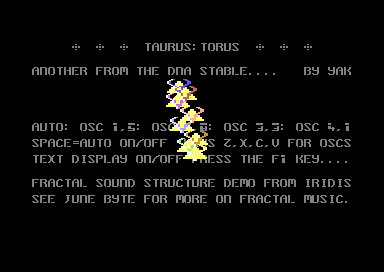
\includegraphics[width=11cm]{torus/torus.png}%
    \end{adjustbox}
}\caption[]{}
\end{figure}

This first demo, released in July 1986(?), has a version of Iridis' music-generating
algorithm that is nearly fully formed. However, the music it produces is quite
different. In fact, it is nearer to a tool for listening to and selecting music than
anything else.

The four seed values in \icode{titleMusicNoteArray} that are used to seed all subequently
generated tunes (\icode{00 07 0C 07} in Iridis Alpha) can be selected and changed by the
user. They're called 'Oscillators' and each can be any value between 0 and 16, i.e. any of
\icode{0 1 2 3 4 5 6 7 8 9 A B C D E F}.


\lstset{style=6502Style}
\lstinputlisting[caption=The music routine in Torus:Taurus side-by-side with Iridis Alpha.,basicstyle=\tiny]{torus/sidebyside.asm}

When it runs the demo cycles through procedural configurations of \icode{titleMusicNoteArray} of 64 notes each.
In other words, exactly the kind of fractal structure we observed in Iridis Alpha proper. The examples below
give a flavour of the music it generats:

\begin{figure}[H]
{
  \begin{adjustbox}{width=14cm,center}
    
\includegraphics[width=14cm]{torus/title_no_1_page_1001.png}}%
  \end{adjustbox}
}\caption[]{Bars 2 and 4 are always repeated}
\end{figure}


\begin{figure}[H]
{
  \begin{adjustbox}{width=14cm,center}
    
\includegraphics[width=14cm]{torus/title_no_2_page_1001.png}}%
  \end{adjustbox}
}\caption[]{Bars 2 and 4 are always repeated}
\end{figure}

Not all of the tunes are 64-note based. It does generate some that are truncated. 

\begin{figure}[H]
  {
    \setlength{\tabcolsep}{3.0pt}
    \setlength\cmidrulewidth{\heavyrulewidth} % Make cmidrule = 
	\centering
	\def\MULTICOLORONE{green}
	\def\MULTICOLORTWO{red}
	\def\SPRITECOLOR{blue}
		
\begin{figure}[H]
  {
    \setlength{\tabcolsep}{3.0pt}
    \setlength\cmidrulewidth{\heavyrulewidth} % Make cmidrule = 
    \begin{adjustbox}{width=3cm,center}
      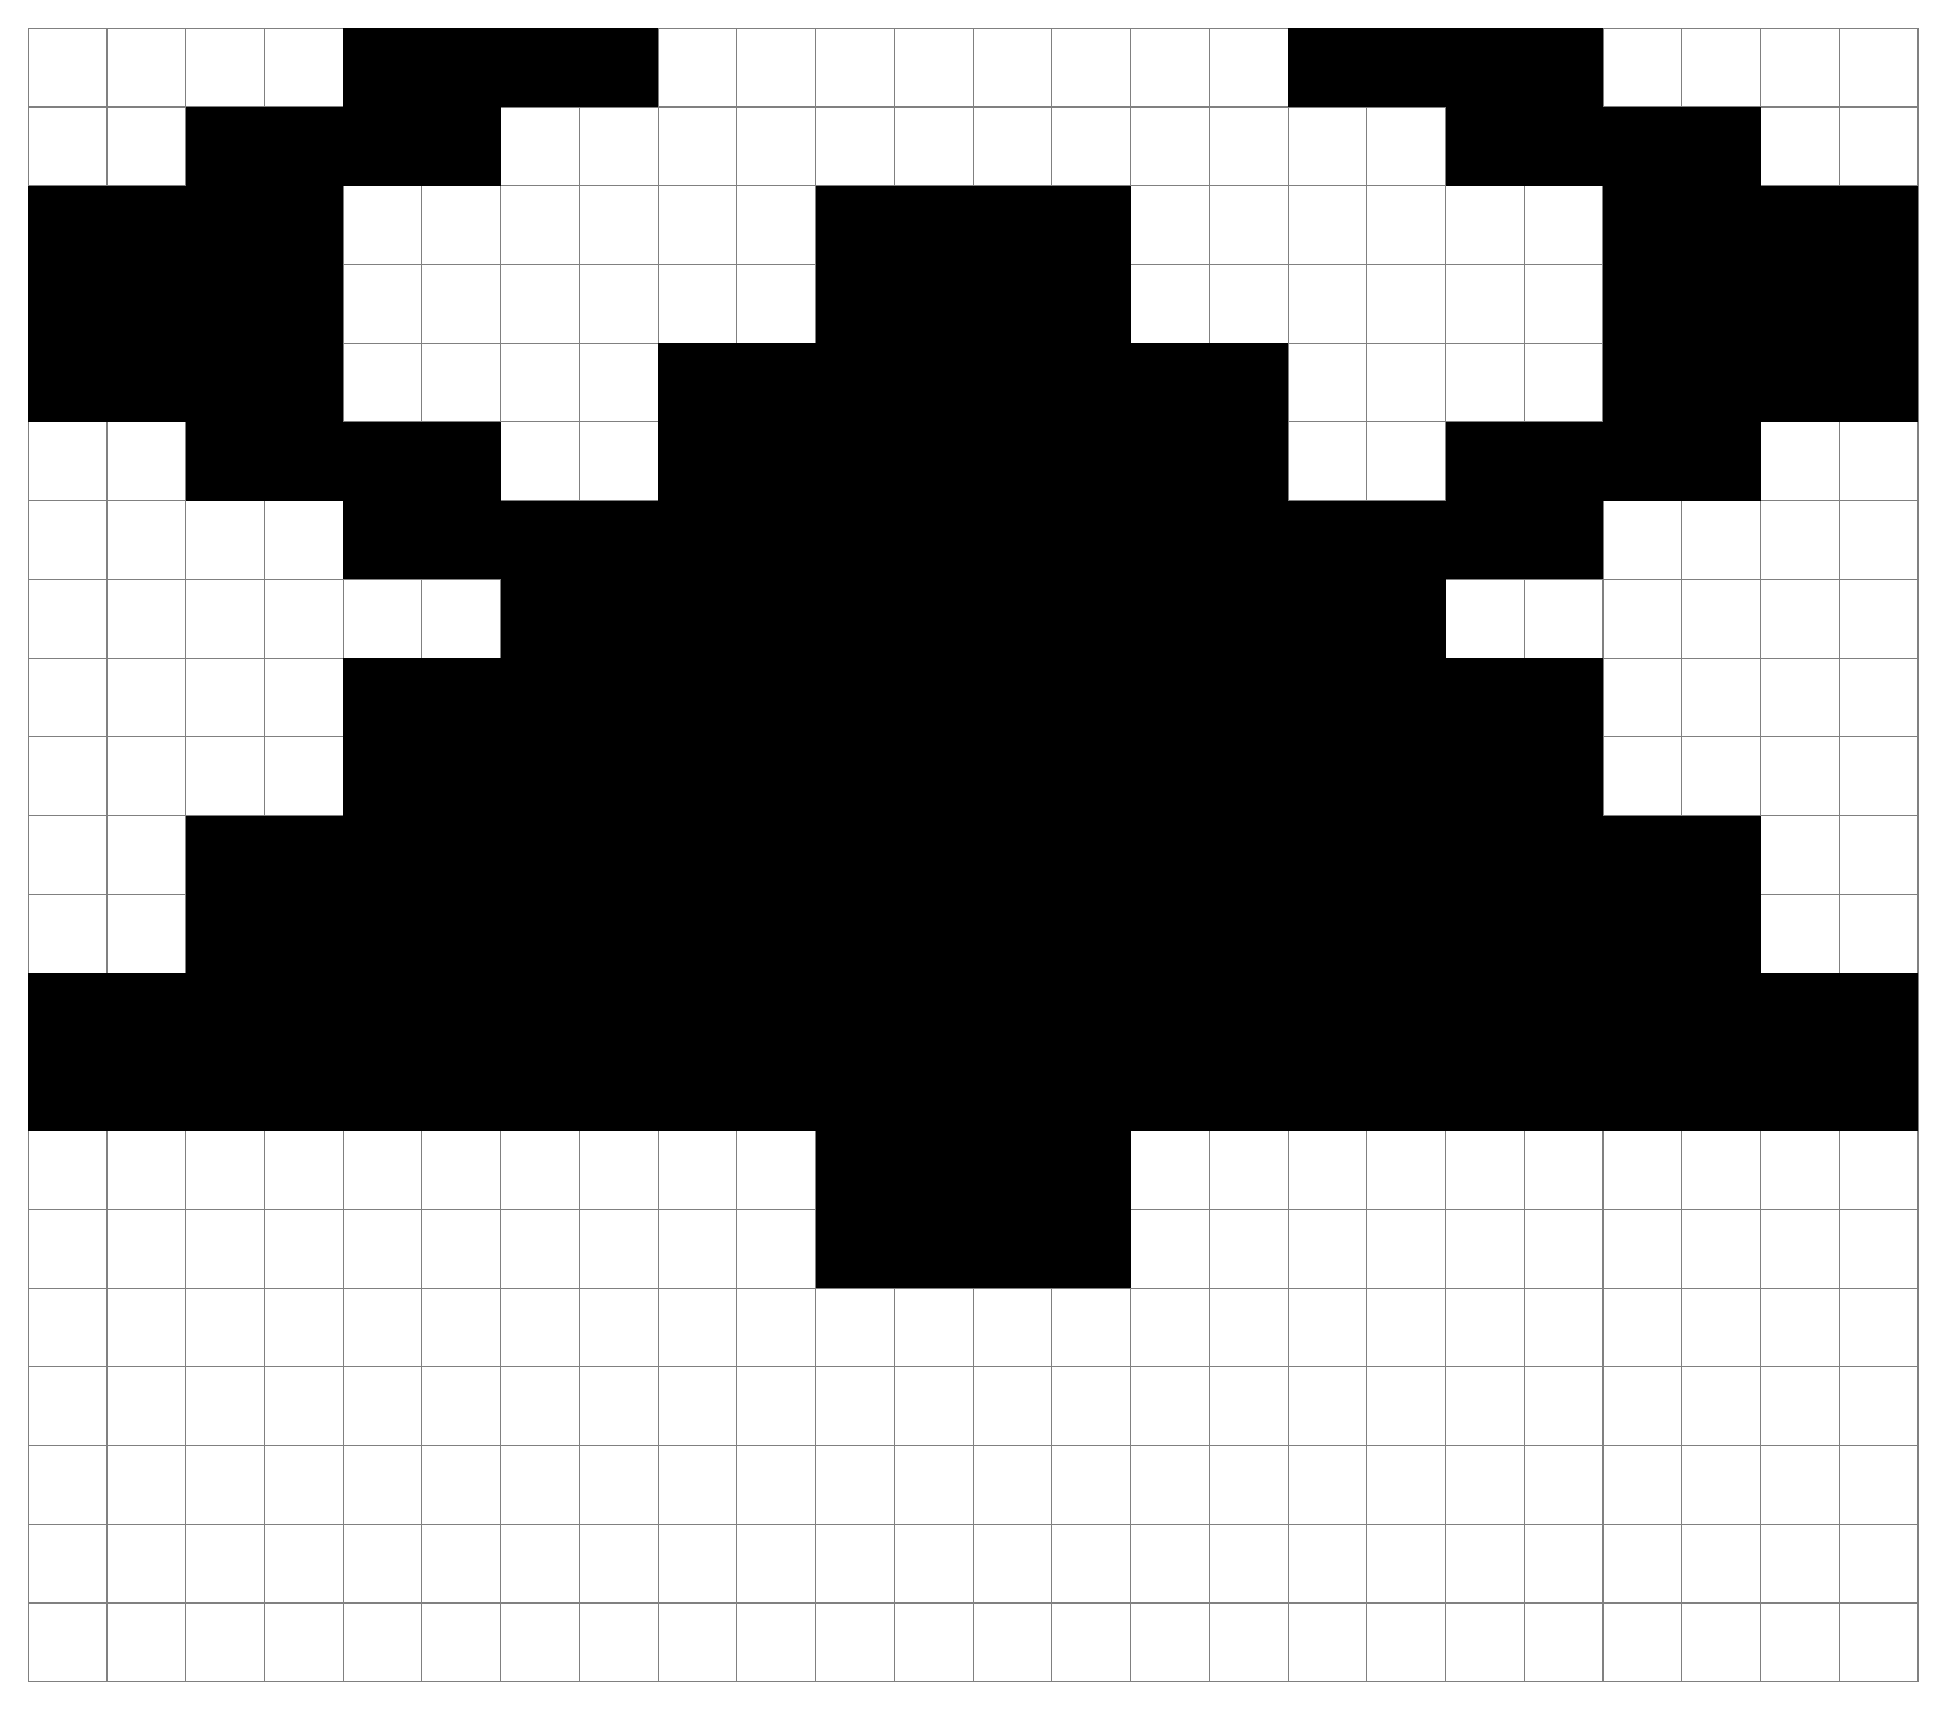
\begin{tikzpicture}

	\draw[step=1.0,gray,thin] (0,0) grid (24,21);
	\fill[\MULTICOLORTWO] (4,20) rectangle ++ (1,1);
	\fill[\MULTICOLORTWO] (5,20) rectangle ++ (1,1);
	\fill[\SPRITECOLOR] (6,20) rectangle ++ (1,1);
	\fill[\SPRITECOLOR] (7,20) rectangle ++ (1,1);
	\fill[\SPRITECOLOR] (16,20) rectangle ++ (1,1);
	\fill[\SPRITECOLOR] (17,20) rectangle ++ (1,1);
	\fill[\SPRITECOLOR] (18,20) rectangle ++ (1,1);
	\fill[\SPRITECOLOR] (19,20) rectangle ++ (1,1);
	\fill[\MULTICOLORTWO] (2,19) rectangle ++ (1,1);
	\fill[\MULTICOLORTWO] (3,19) rectangle ++ (1,1);
	\fill[\SPRITECOLOR] (4,19) rectangle ++ (1,1);
	\fill[\SPRITECOLOR] (5,19) rectangle ++ (1,1);
	\fill[\SPRITECOLOR] (18,19) rectangle ++ (1,1);
	\fill[\SPRITECOLOR] (19,19) rectangle ++ (1,1);
	\fill[\SPRITECOLOR] (20,19) rectangle ++ (1,1);
	\fill[\SPRITECOLOR] (21,19) rectangle ++ (1,1);
	\fill[\MULTICOLORTWO] (0,18) rectangle ++ (1,1);
	\fill[\MULTICOLORTWO] (1,18) rectangle ++ (1,1);
	\fill[\SPRITECOLOR] (2,18) rectangle ++ (1,1);
	\fill[\SPRITECOLOR] (3,18) rectangle ++ (1,1);
	\fill[\MULTICOLORONE] (10,18) rectangle ++ (1,1);
	\fill[\MULTICOLORONE] (11,18) rectangle ++ (1,1);
	\fill[\MULTICOLORONE] (12,18) rectangle ++ (1,1);
	\fill[\MULTICOLORONE] (13,18) rectangle ++ (1,1);
	\fill[\SPRITECOLOR] (20,18) rectangle ++ (1,1);
	\fill[\SPRITECOLOR] (21,18) rectangle ++ (1,1);
	\fill[\SPRITECOLOR] (22,18) rectangle ++ (1,1);
	\fill[\SPRITECOLOR] (23,18) rectangle ++ (1,1);
	\fill[\MULTICOLORTWO] (0,17) rectangle ++ (1,1);
	\fill[\MULTICOLORTWO] (1,17) rectangle ++ (1,1);
	\fill[\SPRITECOLOR] (2,17) rectangle ++ (1,1);
	\fill[\SPRITECOLOR] (3,17) rectangle ++ (1,1);
	\fill[\MULTICOLORONE] (10,17) rectangle ++ (1,1);
	\fill[\MULTICOLORONE] (11,17) rectangle ++ (1,1);
	\fill[\MULTICOLORONE] (12,17) rectangle ++ (1,1);
	\fill[\MULTICOLORONE] (13,17) rectangle ++ (1,1);
	\fill[\SPRITECOLOR] (20,17) rectangle ++ (1,1);
	\fill[\SPRITECOLOR] (21,17) rectangle ++ (1,1);
	\fill[\SPRITECOLOR] (22,17) rectangle ++ (1,1);
	\fill[\SPRITECOLOR] (23,17) rectangle ++ (1,1);
	\fill[\MULTICOLORTWO] (0,16) rectangle ++ (1,1);
	\fill[\MULTICOLORTWO] (1,16) rectangle ++ (1,1);
	\fill[\SPRITECOLOR] (2,16) rectangle ++ (1,1);
	\fill[\SPRITECOLOR] (3,16) rectangle ++ (1,1);
	\fill[\MULTICOLORONE] (8,16) rectangle ++ (1,1);
	\fill[\MULTICOLORONE] (9,16) rectangle ++ (1,1);
	\fill[\MULTICOLORONE] (10,16) rectangle ++ (1,1);
	\fill[\MULTICOLORONE] (11,16) rectangle ++ (1,1);
	\fill[\MULTICOLORONE] (12,16) rectangle ++ (1,1);
	\fill[\MULTICOLORONE] (13,16) rectangle ++ (1,1);
	\fill[\MULTICOLORONE] (14,16) rectangle ++ (1,1);
	\fill[\MULTICOLORONE] (15,16) rectangle ++ (1,1);
	\fill[\SPRITECOLOR] (20,16) rectangle ++ (1,1);
	\fill[\SPRITECOLOR] (21,16) rectangle ++ (1,1);
	\fill[\SPRITECOLOR] (22,16) rectangle ++ (1,1);
	\fill[\SPRITECOLOR] (23,16) rectangle ++ (1,1);
	\fill[\MULTICOLORTWO] (2,15) rectangle ++ (1,1);
	\fill[\MULTICOLORTWO] (3,15) rectangle ++ (1,1);
	\fill[\SPRITECOLOR] (4,15) rectangle ++ (1,1);
	\fill[\SPRITECOLOR] (5,15) rectangle ++ (1,1);
	\fill[\MULTICOLORONE] (8,15) rectangle ++ (1,1);
	\fill[\MULTICOLORONE] (9,15) rectangle ++ (1,1);
	\fill[\MULTICOLORONE] (10,15) rectangle ++ (1,1);
	\fill[\MULTICOLORONE] (11,15) rectangle ++ (1,1);
	\fill[\MULTICOLORONE] (12,15) rectangle ++ (1,1);
	\fill[\MULTICOLORONE] (13,15) rectangle ++ (1,1);
	\fill[\MULTICOLORONE] (14,15) rectangle ++ (1,1);
	\fill[\MULTICOLORONE] (15,15) rectangle ++ (1,1);
	\fill[\SPRITECOLOR] (18,15) rectangle ++ (1,1);
	\fill[\SPRITECOLOR] (19,15) rectangle ++ (1,1);
	\fill[\SPRITECOLOR] (20,15) rectangle ++ (1,1);
	\fill[\SPRITECOLOR] (21,15) rectangle ++ (1,1);
	\fill[\MULTICOLORTWO] (4,14) rectangle ++ (1,1);
	\fill[\MULTICOLORTWO] (5,14) rectangle ++ (1,1);
	\fill[\SPRITECOLOR] (6,14) rectangle ++ (1,1);
	\fill[\SPRITECOLOR] (7,14) rectangle ++ (1,1);
	\fill[\MULTICOLORONE] (8,14) rectangle ++ (1,1);
	\fill[\MULTICOLORONE] (9,14) rectangle ++ (1,1);
	\fill[\MULTICOLORONE] (10,14) rectangle ++ (1,1);
	\fill[\MULTICOLORONE] (11,14) rectangle ++ (1,1);
	\fill[\MULTICOLORONE] (12,14) rectangle ++ (1,1);
	\fill[\MULTICOLORONE] (13,14) rectangle ++ (1,1);
	\fill[\MULTICOLORONE] (14,14) rectangle ++ (1,1);
	\fill[\MULTICOLORONE] (15,14) rectangle ++ (1,1);
	\fill[\SPRITECOLOR] (16,14) rectangle ++ (1,1);
	\fill[\SPRITECOLOR] (17,14) rectangle ++ (1,1);
	\fill[\SPRITECOLOR] (18,14) rectangle ++ (1,1);
	\fill[\SPRITECOLOR] (19,14) rectangle ++ (1,1);
	\fill[\MULTICOLORTWO] (6,13) rectangle ++ (1,1);
	\fill[\MULTICOLORTWO] (7,13) rectangle ++ (1,1);
	\fill[\SPRITECOLOR] (8,13) rectangle ++ (1,1);
	\fill[\SPRITECOLOR] (9,13) rectangle ++ (1,1);
	\fill[\MULTICOLORONE] (10,13) rectangle ++ (1,1);
	\fill[\MULTICOLORONE] (11,13) rectangle ++ (1,1);
	\fill[\MULTICOLORONE] (12,13) rectangle ++ (1,1);
	\fill[\MULTICOLORONE] (13,13) rectangle ++ (1,1);
	\fill[\SPRITECOLOR] (14,13) rectangle ++ (1,1);
	\fill[\SPRITECOLOR] (15,13) rectangle ++ (1,1);
	\fill[\SPRITECOLOR] (16,13) rectangle ++ (1,1);
	\fill[\SPRITECOLOR] (17,13) rectangle ++ (1,1);
	\fill[\MULTICOLORONE] (4,12) rectangle ++ (1,1);
	\fill[\MULTICOLORONE] (5,12) rectangle ++ (1,1);
	\fill[\MULTICOLORTWO] (6,12) rectangle ++ (1,1);
	\fill[\MULTICOLORTWO] (7,12) rectangle ++ (1,1);
	\fill[\SPRITECOLOR] (8,12) rectangle ++ (1,1);
	\fill[\SPRITECOLOR] (9,12) rectangle ++ (1,1);
	\fill[\MULTICOLORONE] (10,12) rectangle ++ (1,1);
	\fill[\MULTICOLORONE] (11,12) rectangle ++ (1,1);
	\fill[\MULTICOLORONE] (12,12) rectangle ++ (1,1);
	\fill[\MULTICOLORONE] (13,12) rectangle ++ (1,1);
	\fill[\SPRITECOLOR] (14,12) rectangle ++ (1,1);
	\fill[\SPRITECOLOR] (15,12) rectangle ++ (1,1);
	\fill[\SPRITECOLOR] (16,12) rectangle ++ (1,1);
	\fill[\SPRITECOLOR] (17,12) rectangle ++ (1,1);
	\fill[\MULTICOLORONE] (18,12) rectangle ++ (1,1);
	\fill[\MULTICOLORONE] (19,12) rectangle ++ (1,1);
	\fill[\MULTICOLORONE] (4,11) rectangle ++ (1,1);
	\fill[\MULTICOLORONE] (5,11) rectangle ++ (1,1);
	\fill[\MULTICOLORTWO] (6,11) rectangle ++ (1,1);
	\fill[\MULTICOLORTWO] (7,11) rectangle ++ (1,1);
	\fill[\SPRITECOLOR] (8,11) rectangle ++ (1,1);
	\fill[\SPRITECOLOR] (9,11) rectangle ++ (1,1);
	\fill[\MULTICOLORONE] (10,11) rectangle ++ (1,1);
	\fill[\MULTICOLORONE] (11,11) rectangle ++ (1,1);
	\fill[\MULTICOLORONE] (12,11) rectangle ++ (1,1);
	\fill[\MULTICOLORONE] (13,11) rectangle ++ (1,1);
	\fill[\SPRITECOLOR] (14,11) rectangle ++ (1,1);
	\fill[\SPRITECOLOR] (15,11) rectangle ++ (1,1);
	\fill[\SPRITECOLOR] (16,11) rectangle ++ (1,1);
	\fill[\SPRITECOLOR] (17,11) rectangle ++ (1,1);
	\fill[\MULTICOLORONE] (18,11) rectangle ++ (1,1);
	\fill[\MULTICOLORONE] (19,11) rectangle ++ (1,1);
	\fill[\MULTICOLORONE] (2,10) rectangle ++ (1,1);
	\fill[\MULTICOLORONE] (3,10) rectangle ++ (1,1);
	\fill[\MULTICOLORONE] (4,10) rectangle ++ (1,1);
	\fill[\MULTICOLORONE] (5,10) rectangle ++ (1,1);
	\fill[\MULTICOLORONE] (6,10) rectangle ++ (1,1);
	\fill[\MULTICOLORONE] (7,10) rectangle ++ (1,1);
	\fill[\MULTICOLORTWO] (8,10) rectangle ++ (1,1);
	\fill[\MULTICOLORTWO] (9,10) rectangle ++ (1,1);
	\fill[\MULTICOLORONE] (10,10) rectangle ++ (1,1);
	\fill[\MULTICOLORONE] (11,10) rectangle ++ (1,1);
	\fill[\MULTICOLORONE] (12,10) rectangle ++ (1,1);
	\fill[\MULTICOLORONE] (13,10) rectangle ++ (1,1);
	\fill[\SPRITECOLOR] (14,10) rectangle ++ (1,1);
	\fill[\SPRITECOLOR] (15,10) rectangle ++ (1,1);
	\fill[\MULTICOLORONE] (16,10) rectangle ++ (1,1);
	\fill[\MULTICOLORONE] (17,10) rectangle ++ (1,1);
	\fill[\MULTICOLORONE] (18,10) rectangle ++ (1,1);
	\fill[\MULTICOLORONE] (19,10) rectangle ++ (1,1);
	\fill[\MULTICOLORONE] (20,10) rectangle ++ (1,1);
	\fill[\MULTICOLORONE] (21,10) rectangle ++ (1,1);
	\fill[\MULTICOLORONE] (2,9) rectangle ++ (1,1);
	\fill[\MULTICOLORONE] (3,9) rectangle ++ (1,1);
	\fill[\MULTICOLORONE] (4,9) rectangle ++ (1,1);
	\fill[\MULTICOLORONE] (5,9) rectangle ++ (1,1);
	\fill[\MULTICOLORONE] (6,9) rectangle ++ (1,1);
	\fill[\MULTICOLORONE] (7,9) rectangle ++ (1,1);
	\fill[\MULTICOLORTWO] (8,9) rectangle ++ (1,1);
	\fill[\MULTICOLORTWO] (9,9) rectangle ++ (1,1);
	\fill[\SPRITECOLOR] (10,9) rectangle ++ (1,1);
	\fill[\SPRITECOLOR] (11,9) rectangle ++ (1,1);
	\fill[\SPRITECOLOR] (12,9) rectangle ++ (1,1);
	\fill[\SPRITECOLOR] (13,9) rectangle ++ (1,1);
	\fill[\SPRITECOLOR] (14,9) rectangle ++ (1,1);
	\fill[\SPRITECOLOR] (15,9) rectangle ++ (1,1);
	\fill[\MULTICOLORONE] (16,9) rectangle ++ (1,1);
	\fill[\MULTICOLORONE] (17,9) rectangle ++ (1,1);
	\fill[\MULTICOLORONE] (18,9) rectangle ++ (1,1);
	\fill[\MULTICOLORONE] (19,9) rectangle ++ (1,1);
	\fill[\MULTICOLORONE] (20,9) rectangle ++ (1,1);
	\fill[\MULTICOLORONE] (21,9) rectangle ++ (1,1);
	\fill[\MULTICOLORONE] (0,8) rectangle ++ (1,1);
	\fill[\MULTICOLORONE] (1,8) rectangle ++ (1,1);
	\fill[\MULTICOLORONE] (2,8) rectangle ++ (1,1);
	\fill[\MULTICOLORONE] (3,8) rectangle ++ (1,1);
	\fill[\MULTICOLORONE] (4,8) rectangle ++ (1,1);
	\fill[\MULTICOLORONE] (5,8) rectangle ++ (1,1);
	\fill[\MULTICOLORONE] (6,8) rectangle ++ (1,1);
	\fill[\MULTICOLORONE] (7,8) rectangle ++ (1,1);
	\fill[\MULTICOLORTWO] (8,8) rectangle ++ (1,1);
	\fill[\MULTICOLORTWO] (9,8) rectangle ++ (1,1);
	\fill[\SPRITECOLOR] (10,8) rectangle ++ (1,1);
	\fill[\SPRITECOLOR] (11,8) rectangle ++ (1,1);
	\fill[\SPRITECOLOR] (12,8) rectangle ++ (1,1);
	\fill[\SPRITECOLOR] (13,8) rectangle ++ (1,1);
	\fill[\SPRITECOLOR] (14,8) rectangle ++ (1,1);
	\fill[\SPRITECOLOR] (15,8) rectangle ++ (1,1);
	\fill[\MULTICOLORONE] (16,8) rectangle ++ (1,1);
	\fill[\MULTICOLORONE] (17,8) rectangle ++ (1,1);
	\fill[\MULTICOLORONE] (18,8) rectangle ++ (1,1);
	\fill[\MULTICOLORONE] (19,8) rectangle ++ (1,1);
	\fill[\MULTICOLORONE] (20,8) rectangle ++ (1,1);
	\fill[\MULTICOLORONE] (21,8) rectangle ++ (1,1);
	\fill[\MULTICOLORONE] (22,8) rectangle ++ (1,1);
	\fill[\MULTICOLORONE] (23,8) rectangle ++ (1,1);
	\fill[\MULTICOLORONE] (0,7) rectangle ++ (1,1);
	\fill[\MULTICOLORONE] (1,7) rectangle ++ (1,1);
	\fill[\MULTICOLORONE] (2,7) rectangle ++ (1,1);
	\fill[\MULTICOLORONE] (3,7) rectangle ++ (1,1);
	\fill[\MULTICOLORONE] (4,7) rectangle ++ (1,1);
	\fill[\MULTICOLORONE] (5,7) rectangle ++ (1,1);
	\fill[\MULTICOLORONE] (6,7) rectangle ++ (1,1);
	\fill[\MULTICOLORONE] (7,7) rectangle ++ (1,1);
	\fill[\MULTICOLORONE] (8,7) rectangle ++ (1,1);
	\fill[\MULTICOLORONE] (9,7) rectangle ++ (1,1);
	\fill[\MULTICOLORTWO] (10,7) rectangle ++ (1,1);
	\fill[\MULTICOLORTWO] (11,7) rectangle ++ (1,1);
	\fill[\SPRITECOLOR] (12,7) rectangle ++ (1,1);
	\fill[\SPRITECOLOR] (13,7) rectangle ++ (1,1);
	\fill[\MULTICOLORONE] (14,7) rectangle ++ (1,1);
	\fill[\MULTICOLORONE] (15,7) rectangle ++ (1,1);
	\fill[\MULTICOLORONE] (16,7) rectangle ++ (1,1);
	\fill[\MULTICOLORONE] (17,7) rectangle ++ (1,1);
	\fill[\MULTICOLORONE] (18,7) rectangle ++ (1,1);
	\fill[\MULTICOLORONE] (19,7) rectangle ++ (1,1);
	\fill[\MULTICOLORONE] (20,7) rectangle ++ (1,1);
	\fill[\MULTICOLORONE] (21,7) rectangle ++ (1,1);
	\fill[\MULTICOLORONE] (22,7) rectangle ++ (1,1);
	\fill[\MULTICOLORONE] (23,7) rectangle ++ (1,1);
	\fill[\MULTICOLORTWO] (10,6) rectangle ++ (1,1);
	\fill[\MULTICOLORTWO] (11,6) rectangle ++ (1,1);
	\fill[\SPRITECOLOR] (12,6) rectangle ++ (1,1);
	\fill[\SPRITECOLOR] (13,6) rectangle ++ (1,1);
	\fill[\MULTICOLORTWO] (10,5) rectangle ++ (1,1);
	\fill[\MULTICOLORTWO] (11,5) rectangle ++ (1,1);
	\fill[\SPRITECOLOR] (12,5) rectangle ++ (1,1);
	\fill[\SPRITECOLOR] (13,5) rectangle ++ (1,1);

      \end{tikzpicture}
    \end{adjustbox}
  }\caption{BULLHEAD}
\end{figure}

  }\caption[position=top]{The 'Torus' sprite.}
\end{figure}


\subsection{Taurus/Torus Two}
\begin{figure}[H]
{
  \begin{adjustbox}{width=11cm,center}
  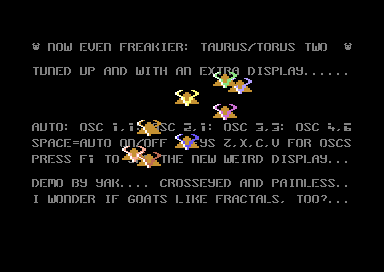
\includegraphics[width=11cm]{torus/torus2.png}%
    \end{adjustbox}
}\caption[]{}
\end{figure}

\lstset{style=6502Style}
\lstinputlisting[caption=The music routine in Taurus:Torus II side-by-side with Iridis Alpha.,basicstyle=\tiny]{torus/sidebyside2.asm}


\begin{figure}[H]
{
  \begin{adjustbox}{width=14cm,center}
    
\includegraphics[width=14cm]{torus/torus2_title_no_1_page_1001.png}%
  \end{adjustbox}
}\caption[]{}
\end{figure}

\begin{figure}[H]
{
  \begin{adjustbox}{width=14cm,center}
    
\includegraphics[width=14cm]{music/title_no_1_page_1001.png}%
  \end{adjustbox}
}\caption[]{}
\end{figure}

\subsection{Making the Bonus Bounty Animation}
\begin{figure}[H]
{
  \setlength{\tabcolsep}{3.0pt}
  \setlength\cmidrulewidth{\heavyrulewidth} % Make cmidrule = 
    \begin{adjustbox}{width=12cm,center}
  \begin{subfigure}{0.3\textwidth}
  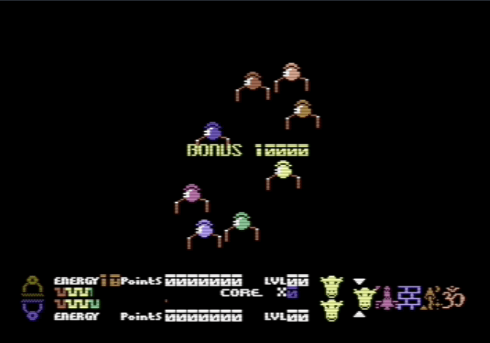
\includegraphics[width=4cm]{torus/bonusbounty.png}%
  \end{subfigure}
  \begin{subfigure}{0.3\textwidth}
  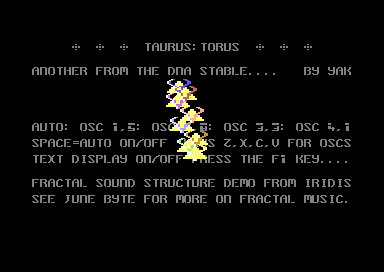
\includegraphics[width=4cm]{torus/torus.png}%
  \end{subfigure}
  \end{adjustbox}
}\caption[]{The Torus oscillator animation and Iridis' bonus animation.}
\end{figure}

The Torus demo is also where the elegant animation used when awarding a bonus was developed. The code
handling each is identical and was only very lightly modified for the final game.

\begin{minipage}[b]{0.45\linewidth}
\centering
\CopyPartialFile{../iridisalpha/demos/torus/src/torus.asm}{tmp.asm}{361}{412}%
\lstinputlisting[caption=Animation in Torus Demo,basicstyle=\tiny]{tmp.asm}
\end{minipage}
\hspace{0.5cm}
\begin{minipage}[b]{0.45\linewidth}
\centering
\CopyPartialFile{../iridisalpha/src/iridisalpha.asm}{tmp.asm}{5055}{5106}%
\lstinputlisting[caption=... and Iridis Alpha,basicstyle=\tiny]{tmp.asm}
\end{minipage}


\begin{tcolorbox}[%
  breakable,
  parbox = false,
  frame hidden,
  sharp corners,
  after skip=10pt,
  overlay broken = {
    \draw[]
      (frame.north west) rectangle (frame.south east);},
]{}
A Testing Hack

In the CheckKeyboardInGame Routine, we find the following:
\CopyPartialFile{../iridisalpha/src/iridisalpha.asm}{tmp.asm}{7909}{7920}%
\lstinputlisting[basicstyle=\tiny]{tmp.asm}

In the above the `canAwardBonus` byte is the first letter in the name of the player with the top score in the Hi-Score table. By default this is 'YAK':
\CopyPartialFile{../iridisalpha/src/iridisalpha.asm}{tmp.asm}{8713}{8716}%
\lstinputlisting[basicstyle=\tiny]{tmp.asm}

But if we change 'Y' to \icode{\$1C} like so, we can activate the hack:

\begin{lstlisting}[basicstyle=\tiny]
hiScoreTablePtr           .TEXT "0068000"
canAwardBonus             .TEXT $1C,"AK "
\end{lstlisting}

Note that \icode{\$1C} is charset code for a bull's head symbol in Iridis Alpha, so it is also possible to enter this as the initial of a high scorer name if we get a score that puts us to the top of the table:

\CopyPartialFile{../iridisalpha/src/graphics/charset.asm}{tmp.asm}{287}{296}%
\lstinputlisting[basicstyle=\tiny]{tmp.asm}


I'm guessing this was used for testing the animation routine and left in as an Easter egg.



\end{tcolorbox}%
